\section{Development Environment}

Our development environment is built for consistency, scalability, and security. We use Orbstack to manage all containers, making setup and code syncing easy.

\subsection{Backend Containers}
The backend is structured as follows:
\begin{itemize}
    \item \textbf{Nginx + PHP-FPM + XHProf Container:} Runs the Drupal code, serves the application, handles all web requests, and provides profiling/debugging with XHProf. Code is synced from the host using Orbstack.
    \item \textbf{Memcached Container:} Connected to the main container for backend caching, improving speed and performance.
    \item \textbf{MySQL Container:} Stores all structured data for Drupal, connected internally to the main container and PhpMyAdmin.
    \item \textbf{PhpMyAdmin Container:} Provides a GUI for managing the MySQL database.
    \item \textbf{Mailhog Container:} Used for email testing. Drupal is configured to send emails via SMTP to Mailhog, which catches them for testing.
\end{itemize}

- Ports are exposed as follows: Drupal (8080), PhpMyAdmin (8085), Mailhog (8002).
- Database and Memcached containers are only accessible via the internal Docker network for security.

\subsection{Frontend Containers}
The frontend setup includes:
\begin{itemize}
    \item \textbf{Node.js Container:} Runs the Next.js application.
    \item \textbf{Redis Container:} Used for caching and boosting frontend performance.
    \item \textbf{Redis Commander Container:} Allows management of Redis cache via terminal or GUI.
\end{itemize}

The Next.js frontend communicates with the backend, but a reverse proxy is set up so the backend is not directly exposed. All API requests go through the frontend, making the backend invisible to the outside.

% \subsection{Frontend-Backend Decoupling}

% The platform's architecture is fully decoupled \cite{richardson2018microservices}. The frontend and backend run as separate services, communicating only through JSON:API. Drupal's native support for this standard meant we didn't have to build custom endpoints for every entity—content, taxonomies, users, and files were all exposed automatically, with permissions handled by Drupal itself. for example:
% \begin{itemize}
%   \item Content Types: \texttt{/jsonapi/node/\{type\}}
%   \item Taxonomies: \texttt{/jsonapi/taxonomy\_term/\{vocabulary\}}
%   \item Users: \texttt{/jsonapi/user/user}
%   \item Files: \texttt{/jsonapi/file/file}
% \end{itemize}

\subsubsection{Widget-Based Component Binding}

To empower non-technical users, we built a widget system in Drupal. Each widget comes with a \textbf{screenshot}, a \textbf{.twig} template for monolithic deployments, and a \textbf{settings.yml} for the decoupled frontend. On the Next.js side, a webpack plugin scans for \textbf{*Widget.jsx} files, reads their metadata, and links them to backend widgets. This setup allows for lazy loading and keeps the bundle size in check.

\subsubsection{Route Translation and UUID Resolution}

SEO-friendly URLs are a must. Using Drupal's Pathauto, every alias (like /internship-offers) is mapped to a UUID and content type. The frontend then fetches the right data via JSON:API, so routing stays flexible and isn't tied to backend structure.
Here is an example of a route translation:
\begin{enumerate}
  \item The alias (e.g., \texttt{/internship-offers}) is passed to a translation endpoint.
  \item A response returns the \texttt{UUID} and \texttt{content type}.
  \item The UUID is used to fetch detailed JSON:API data for rendering.
\end{enumerate}

\subsection{Secure API Proxying}

Direct backend exposure is risky. All API calls go through a Next.js proxy endpoint, which lets us tweak headers, strip cookies, and add caching or rate limits if needed. This extra layer keeps things secure and gives more control over traffic.

\subsection{Caching Architecture}

Performance matters, especially as the platform grows. We set up Memcached on the Drupal side for dynamic content and Redis on the frontend for frequently accessed collections and sessions. Redis Commander makes it easy to inspect and debug cache contents.

\subsection{Mail Testing Infrastructure}

Testing email flows without spamming real users is crucial. MailHog catches all outgoing mail in the dev stack, so we can check templates and triggers safely.

\subsection{Component Development with Storybook}

Storybook runs in its own container, letting us and the team build and preview UI components in isolation. Mocked backend data and stakeholder previews help us catch design issues early.
\begin{figure}[H]
  \centering
  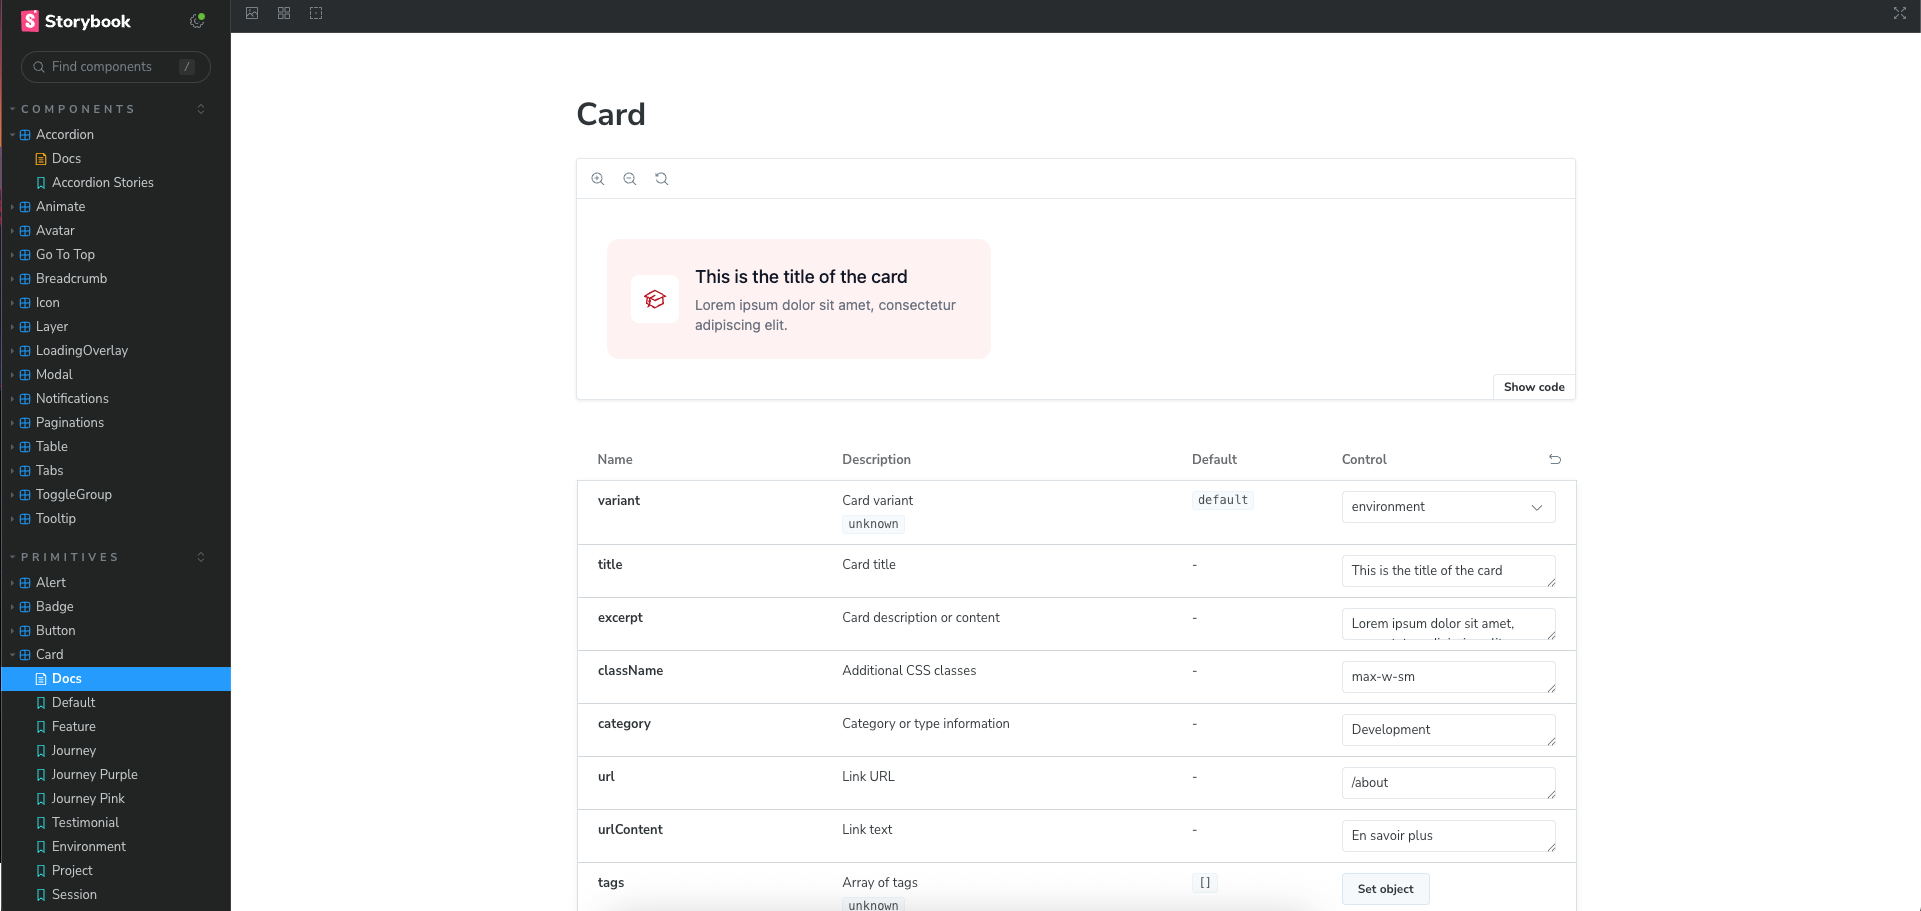
\includegraphics[width=\textwidth]{images/storybook.png}
  \caption{Storybook UI}
  \label{fig:storybook}
\end{figure}


\subsection{Routing Strategy}

We opted for Next.js Pages Router over the newer App Router. The Pages Router is stable, well-documented, and better supported by the modules we needed. Data fetching is straightforward, and the learning curve is lower for new contributors.
